\documentclass[sigconf]{acmart}
\usepackage{booktabs}
\usepackage{siunitx}

%% \BibTeX command to typeset BibTeX logo in the docs
\AtBeginDocument{%
  \providecommand\BibTeX{{%
    \normalfont B\kern-0.5em{\scshape i\kern-0.25em b}\kern-0.8em\TeX}}}

\DeclareMathOperator*{\argmax}{argmax}
\DeclareMathOperator*{\argmin}{argmin}

%% These commands are for a PROCEEDINGS abstract or paper.
\settopmatter{printacmref=false} % Removes citation information below abstract
\renewcommand\footnotetextcopyrightpermission[1]{} % removes footnote with conference information in 

\acmConference[AEPRO 2026]{AEPRO 2026: Algorithm Engineering Projects}{March 16}{Jena, Germany}

% convert text to title case
% http://individed.com/code/to-title-case/

% that helps you to formulate your sentences
% https://www.deepl.com/translator

\begin{document}

%%
%% The "title" command has an optional parameter,
%% allowing the author to define a "short title" to be used in page headers.
\title[pytotune: An Efficient Open-Source Auto-Tune Python Library]{pytotune: An Efficient Open-Source Auto-Tune Python Library\\\large Algorithm Engineering 2026 Project Paper}

%%
%% The "author" command and its associated commands are used to define
%% the authors and their affiliations.

\author{Hannes Spitz}
\affiliation{%
  \institution{Friedrich Schiller University Jena}
  \country{Germany}}
\email{hannes.spitz@uni-jena.de}

\author{Moritz Seppelt}
\affiliation{%
  \institution{Friedrich Schiller University Jena}
  \country{Germany}}
\email{moritz.seppelt@uni-jena.de}

%% The abstract is a short summary of the work to be presented in the article.
\begin{abstract}

The five-finger pattern \cite{macgilchrist2014}:
\begin{enumerate}
\item \textbf{Topic and background:} What topic does the paper deal with? What is the point of departure for your research? Why are you studying this now?
\item \textbf{Focus:} What is your research question? What are you studying precisely?
\item \textbf{Method:} What did you do?
\item \textbf{Key findings:} What did you discover?
\item \textbf{Conclusions or implications:} What do these findings mean? What broader issues do they speak to?
\end{enumerate}


\end{abstract}

%%
%% Keywords. The author(s) should pick words that accurately describe
%% the work being presented. Separate the keywords with commas.
\keywords{entity resolution, data cleansing, programming contest}


%%
%% This command processes the author and affiliation and title
%% information and builds the first part of the formatted document.
\maketitle

\let\thefootnote\relax\footnotetext{AEPRO 2026, March 1, Jena, Germany. Copyright \copyright 2026 for this paper by its authors. Use permitted under Creative Commons License Attribution 4.0 International (CC BY 4.0).}


\section{Introduction}
Pitch correction, commonly known as Auto-Tune, is a signal processing task in which the fundamental frequency of an audio signal is estimated and adjusted to match a predefined musical target. Formally, given a time-domain audio signal, the system must extract its pitch trajectory and map it to a discrete set of target frequencies defined by a MIDI sequence or by a musical scale. This problem combines frequency estimation, discrete mapping, and signal transformation within a single algorithmic pipeline. While Python provides powerful tools for audio analysis, there are comparatively few open-source libraries that offer an integrated, installable pitch correction solution with a performance-oriented backend and flexible tuning support. One example might be \texttt{py-autotune} \cite{py_autotune_pypi}, although it does not seam to be developed with performance in mind.

In this project, we develop an open-source pitch correction library with a C++ core and a Python interface, designed for distribution via PyPI. The goal is to provide a reusable and accessible tool that integrates efficiently into Python-based audio workflows while leveraging the computational advantages of C++ for the core processing steps. 
Publishing the library as an installable package emphasizes reproducibility, transparency, and practical usability beyond a prototype implementation.

The system supports two modes of operation. In the first mode, an audio file is corrected according to a corresponding MIDI file, allowing explicit control of the target pitch over time. In the second mode, detected pitches are quantized to a user-defined scale relative to a reference tuning (e.g., A4 = 440 Hz). The design allows flexible pitch sets, including scales that do not necessarily repeat within a single octave, thereby generalizing beyond conventional 12-tone systems.

The focus of this work lies in the systematic engineering of the algorithmic pipeline. Beyond defining clear input specifications and modularizing pitch detection and pitch shifting components, we evaluated the implementation empirically to identify performance bottlenecks. Based on these measurements, critical sections were refined and optimized within the C++ backend, while maintaining a clean Python API suitable for open-source distribution via PyPI. This iterative process of implementation, measurement, and targeted improvement reflects the core principles of algorithm engineering.

% % \subsection{Background}

\subsection{Related Work}
Pitch correction has been studied extensively in both industry and academia due to its widespread application in music production \cite{diaz2009fate}. Commercial plugins such as Antares Auto-Tune \cite{antares_autotune_website} have become standard tools in professional studios, implementing complex pitch estimation and correction strategies that are optimized for perceptual quality and real-time performance. In addition to traditional signal-processing techniques, recent research has explored machine learning approaches to pitch tracking and correction , including deep neural networks \cite{wager2020deep} trained to estimate fundamental frequency or directly synthesize pitch-shifted audio. These data-driven methods can achieve impressive accuracy in challenging acoustic conditions, but they often sacrifice transparency and interpretability, making it difficult to analyze or adapt their internal behavior without access to training data and model details.

In contrast to data-driven systems, classic algorithmic methods such as autocorrelation \cite{upadhya2012pitch}, cepstral analysis \cite{noll1967cepstrum}, and spectral estimation \cite{vincent2009adaptive} remain foundational in fundamental frequency detection. Among these, the YIN algorithm \cite{de2002yin} is a well-validated approach \cite{sukhostat2015comparative} that estimates pitch by minimizing a difference function derived from the autocorrelation of the signal, providing good stability across a wide range of monophonic inputs.

For the pitch-shifting step, there exist multiple strategies ranging from time-domain resampling \cite{laroche2002time} to phase vocoder techniques \cite{flanagan1966phase}. Bernsee’s Fourier-transform-based \cite{bernsee_pitch_shifting_ft} method implements pitch shifting by manipulating spectral bins while preserving phase relationships, offering a practical compromise between audio quality and computational cost.

Our project targets a middle path between highly engineered commercial products and opaque machine learning models. We wanted a solution whose behavior we can trace end-to-end and whose performance characteristics we can measure and optimize systematically. To that end, we selected the YIN algorithm for pitch detection and Bernsee’s Fourier-based pitch shifter for pitch modification. These choices reflect a preference for algorithmic transparency, reproducibility, and the ability to reason precisely about the processing pipeline, which supports our goals of trackability and open-source distribution.


% \subsection{Our Contributions}

\subsection{Outline}
The paper is structured as follows. First, we introduce our pitch correction algorithm and describe each stage of the processing pipeline. Next, we highlight the points in the algorithm where profiling revealed optimization opportunities, specifying which were implemented and which were deemed non-critical due to low impact on overall performance. This is followed by a presentation of our experimental results, including measurements of the effectiveness of implemented optimizations and a detailed bottleneck analysis. Finally, we summarize our findings and conclusions.

\section{Mode of Operation}
The development process followed an agile-inspired workflow with loosely structured sprints complemented by regular meetings to coordinate tasks and track progress. Algorithmic components were initially implemented in a straightforward manner, then profiled and optimized iteratively. We were able to benchmark the performance improvements across macOS and Linux.

Profiling tools such as Intel VTune Profiler and Xcode Instruments were employed to identify computational bottlenecks. Targeted optimizations were subsequently applied to critical sections of the C++ backend, improving execution efficiency while maintaining correctness.

Testing was conducted using the Google Test framework (GTest) to ensure functionality and stability throughout the development cycle and on the different plattforms Windows, MacOS and Linux. Build configuration and compilation were managed with CMake, while Python bindings were implemented using pybind11 to provide a seamless interface. Parallelization opportunities and other optimization stratigies were explored using OpenMP and vectorization using Highway \cite{highway}

\section{The Algorithm}
\textbf{Auch beschreibe Optimierungen, die möglich wären, aber weil kein Bottle Neck nicht gemacht haben.}

\subsection{The Pipeline}
The processing pipeline begins by reading the input audio file and, if applicable, a corresponding MIDI file. The audio is then divided into short windows, and the YIN algorithm is applied to estimate the pitch for each segment. Target pitches are determined either from the MIDI data or a user-defined scale. Finally, each window is pitch-corrected using Bernsee’s Fourier-based algorithm, and the corrected segments are overlapped and combined to synthesize the final output signal.

A basic concept that we pass through the whole pipeline is \texttt{Windowing}. This represents the assignment of samples of the sound file to overlapping sections, which we call windows. Typically, one value is assigned to multiple adjacent windows. All pitch detection and shifting is then performed on this grid. The overlap is important for smoothing out the edges when the windows are recombined. For that Hann Windows are used \cite[Chapter~13.4, p.~657]{press2007numerical}. Our default windowing has a width of $4096$ samples (at a typical sample rate of \SI{44.1}{\kilo\hertz}, this represents \SI{92.9}{\milli\second}) and a stride of $1024$ values.

\begin{figure}[h]  % "h" means place here (approx)
    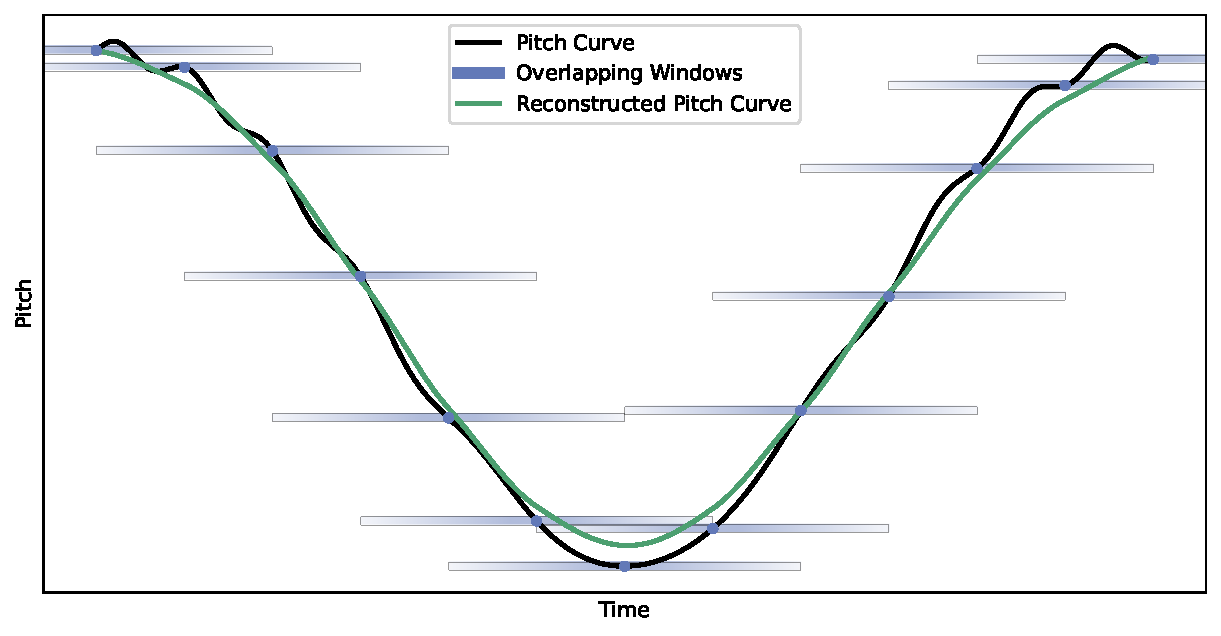
\includegraphics[width=0.4\textwidth]{graphics/windowing.pdf} % adjust width
    \caption{Illustration of the overlapping windowing and pitch reconstruction. Window opacity indicates each window's contribution to the reconstructed pitch using Hann windows.}
    \label{fig:windowing}
\end{figure}

\subsection{Input Processing}
\subsubsection{File formats}
Standard implementations were used to read and write audio and MIDI files without any special optimisation. WAV files were loaded to extract raw sample data and MIDI files were parsed to obtain note events and timing information. This information was then converted into windowed data, i.e. which note plays at a particular window. This step contributes negligibly to the program's overall runtime. (see Section~\ref{sec:experiments}).

\subsubsection{Scale}
\label{sec:scale}
In the code, a musical scale is represented by a \texttt{float baseNote}, which is the pitch of a base note, the \texttt{float[] notes} represent the factor by which the baseNote has to be multiplied to get the note pitches, and the \texttt{float repeatFactor} is the multiplicative factor between adjacent \texttt{baseNotes}. The latter is most commonly set to 2, representing one octave. Note that pitches live on a logarithmic scale, so all distances are multiplicative. Thus, the set of all notes in scale $S$ becomes:
$$S = \{r^k \cdot b \cdot n\mid m \in \mathbb{Z}, n \in N\}$$
with the \texttt{baseNote} $b$, the \texttt{repeatFactor} $r$, the set of \texttt{notes} $N$ and the octave $k$.

The algorithmic problem we had to face, was given some pitch $f$ find the closest pitch $f' \in S$, basically projecting $f$ on $S$. The projection is given by
$$\pi(f) = \argmin_{f'\in S} \max\left\{\frac{f}{f'}, \frac{f'}{f}\right\} = \argmin_{f'\in S}|\log f - \log f'|$$

We solved this by first determining the octave that $f$ is in, and then using a linear search to obtain the neighbouring notes. Finally, we compared the distances and returned the closer note. A binary search would also be possible, offering a theoretical improvement, but as most scales include fewer than twenty notes, the practical improvement would be negligible.

\subsection{Pitch Detection}
\label{sec:pitch-detection}
\subsubsection{The YIN Algorithm}
\subsubsection{Optimisations}
- Wir wissen es gibt noch eine FFT Variante, aber haben wir geskippt. Mit Citation und Möglicher Verbesserung

- Downsampling

- Parallalisation

\subsection{Pitch Correction}
In \ref{sec:pitch-detection} we detected some pitch $f_m$ for each window $m$, and dependent on the mode, we can extract the target pitch $f'_m$ from the midi file or by projecting onto a scale (see \ref{sec:scale}). Now it is left to shift up the pitch of the window by $\alpha_m := \frac{f'_m}{f_m}$.
\subsubsection{The Algorithm}
We took the algorithm from Staphan Bernsee's Blog on \textit{Pitch Shifting Using The Fourier Transform} \cite{bernsee_pitch_shifting_ft}. As he already discribed the algorithm in detail, let's just revisit the most important deatils.

The core idea of the pitch shifting algorithm is conceptually simple: each segment of the signal is transformed to the frequency domain using a descrete Fourier transform (DFT), the frequencies are scaled by the desired pitch factor $\alpha_m$, and then the signal is reconstructed with an inverse Fourier transform. In other words, for a windowed frame $x[n]$, one could naively attempt
$$
\tilde{x}[n] = \text{DFT}^{-1}\left(\text{DFT}(x[n]) \big|_{k \mapsto \alpha_m k}\right)
$$

However, directly scaling frequency bins in this way ignores the phase relationships between successive frames. Here, each \emph{bin} corresponds to a discrete frequency component of the Fourier transform, representing the amplitude and phase of a narrow frequency band. Simply reassigning magnitudes to new bins would produce discontinuities in the waveform, resulting in strong artifacts such as beating or phasiness.

To avoid this, the algorithm keeps track of the instantaneous phase of each frequency component. Let $X_m[k] = |X_m[k]| e^{j \phi_m[k]}$ be the DFT of the $m$-th windowed frame. The phase difference between successive frames,
$$
\Delta \varphi_m[k] = \varphi_m[k] - \varphi_{m-1}[k],
$$
is computed and compared against the expected phase advance for that bin based on the window stride. This allows the true instantaneous frequency to be estimated:
$$
\omega_m[k] = \frac{2 \pi k}{W} + \frac{\Delta \varphi_m[k] - 2 \pi k R / W}{R},
$$
which represents the actual frequency content rather than the discrete bin location.

By scaling these instantaneous frequencies instead of naïvely moving bins, the algorithm preserves temporal continuity. The scaled magnitudes are then reassigned to the corresponding bins in the synthesis frame, the phases are updated accordingly, and the inverse DFT reconstructs the time-domain signal.

\subsubsection{Optimisations}


\section{Experiments}

\subsection{Bottleneck Analysis}
\subsection{Optimization Comparisson}
Table~\ref{tab:results} shows the running times of the resolution step of the five best placed teams.


\begin{table}[htbp]
  \caption{Comparison of the F-measure and the running times of the resolution step of the five best placed teams. The input data for the resolution step consisted of 29{,}787 in JSON formatted e-commerce websites. Measurements were taken on a
laptop running Ubuntu 19.04 with 16 GB of RAM and two Intel Core i5-4310U CPUs. The underlying SSD was a 500\,GB 860 EVO mSATA. We cleared the page cache, dentries, and inodes before each run to avoid reading the input data from RAM instead of the SSD.}
  \label{tab:results}
\resizebox{\columnwidth}{!}{
  \begin{tabular}{lcrr}
    \toprule
    Team& Language & F-measure & Running time (s)\\
    \midrule
	PictureMe (\textbf{this paper}) &C++& 0.99 & \textbf{0.61}\\
    DBGroup@UniMoRe &Python& 0.99 & 10.65\\
    DBGroup@SUSTech &C++& 0.99 & 22.13\\
    eats\_shoots\_and\_leaves &Python& 0.99 & 28.66\\
    DBTHU &Python& 0.99& 63.21\\
  \bottomrule
\end{tabular}
}
\end{table}


\section{Conclusions}

%%
%% The next two lines define the bibliography style to be used, and
%% the bibliography file.
\bibliographystyle{ACM-Reference-Format}
\bibliography{literature}


\end{document}
\endinput
%%
%% End of file `sample-sigconf.tex'.
